\documentclass{article}
\usepackage{color}
\usepackage{amssymb}
\usepackage{xcolor}
\usepackage{pgfplots}
\pgfplotsset{compat = newest}
\usepgfplotslibrary{fillbetween}

\begin{document}

   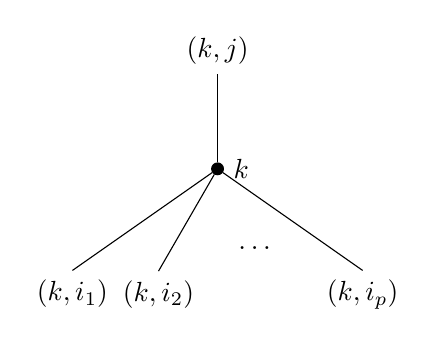
\begin{tikzpicture}
% Creating a small black node
  \node[circle, draw, fill=black, inner sep=1.5pt] (myNode) at (0,0) {};
% Adding label next to the node with math expression
  \node[right] at (myNode.east) {$k$}; 
  % Drawing edges
  \draw[-] (myNode) -- ++(90:1.2cm) node[midway, above, pos=1.0] {$(k,j)$};
  \draw[-] (myNode) -- ++(215:2.25cm) node[midway, below, pos=1.0] {$(k,i_1)$};
    \draw[-] (myNode) -- ++(240:1.5cm) node[midway, below, pos=1.0] {$(k,i_2)$};
  \draw[-] (myNode) -- ++(325:2.25cm) node[midway, below, pos=1.0] {$(k,i_p)$};
   % Adding horizontal dots at specified coordinates
  \node at (.5,-1) {\ldots};
\end{tikzpicture}

\end{document}